\section{Results}
\label{Results}

We ran the Tamarin prover version 1.4.1 in automatic mode to prove the 4 lemmata presented above. The verification took 20,158s on a Ubuntu 18.04 Laptop with an Intel(R) Core(TM) i7-8650U CPU and 16GB of RAM. All 4 lemmata could be verified without interaction. The source code of the Tamarin model is available for download at GitHub\footnote{https://github.com/kr4ck-com/LDACS-MAKE} and can be found in Appendix \ref{TamarinCode}.

In Table \ref{tab:tamarin_results} we present the Tamarin output for each lemma. The scope column states which type of proof has been done: 'exists-trace'-proofs verify, that the given property or lemma holds at least for one trace of the protocol; 'all-traces'-proofs respectively verify that the property holds for all protocol traces. The last column gives the number of verification steps that were executed by Tamarin to verify the appropriate lemma. As can be seen, the "Secure Key Exchange"-lemma took substantially more steps than the others to be verified.

\begin{table}
	\centering
    \caption{Verification results for the LDACS MAKE protocol}
    \begin{tabular}{|l|c|c|r|}
    \hline
        Lemma & Scope & Result & Steps \\
        \hline
        Executable & exists-trace & verified & 21 \\
        Secure Key Exchange & all-traces & verified & 615 \\
        Perfect Forward Secrecy & all-traces & verified & 19 \\
        Mutual Authentication & all-traces & verified & 29 \\
        
        \hline
    \end{tabular}
    
    \label{tab:tamarin_results}
\end{table}
 
\begin{figure}
		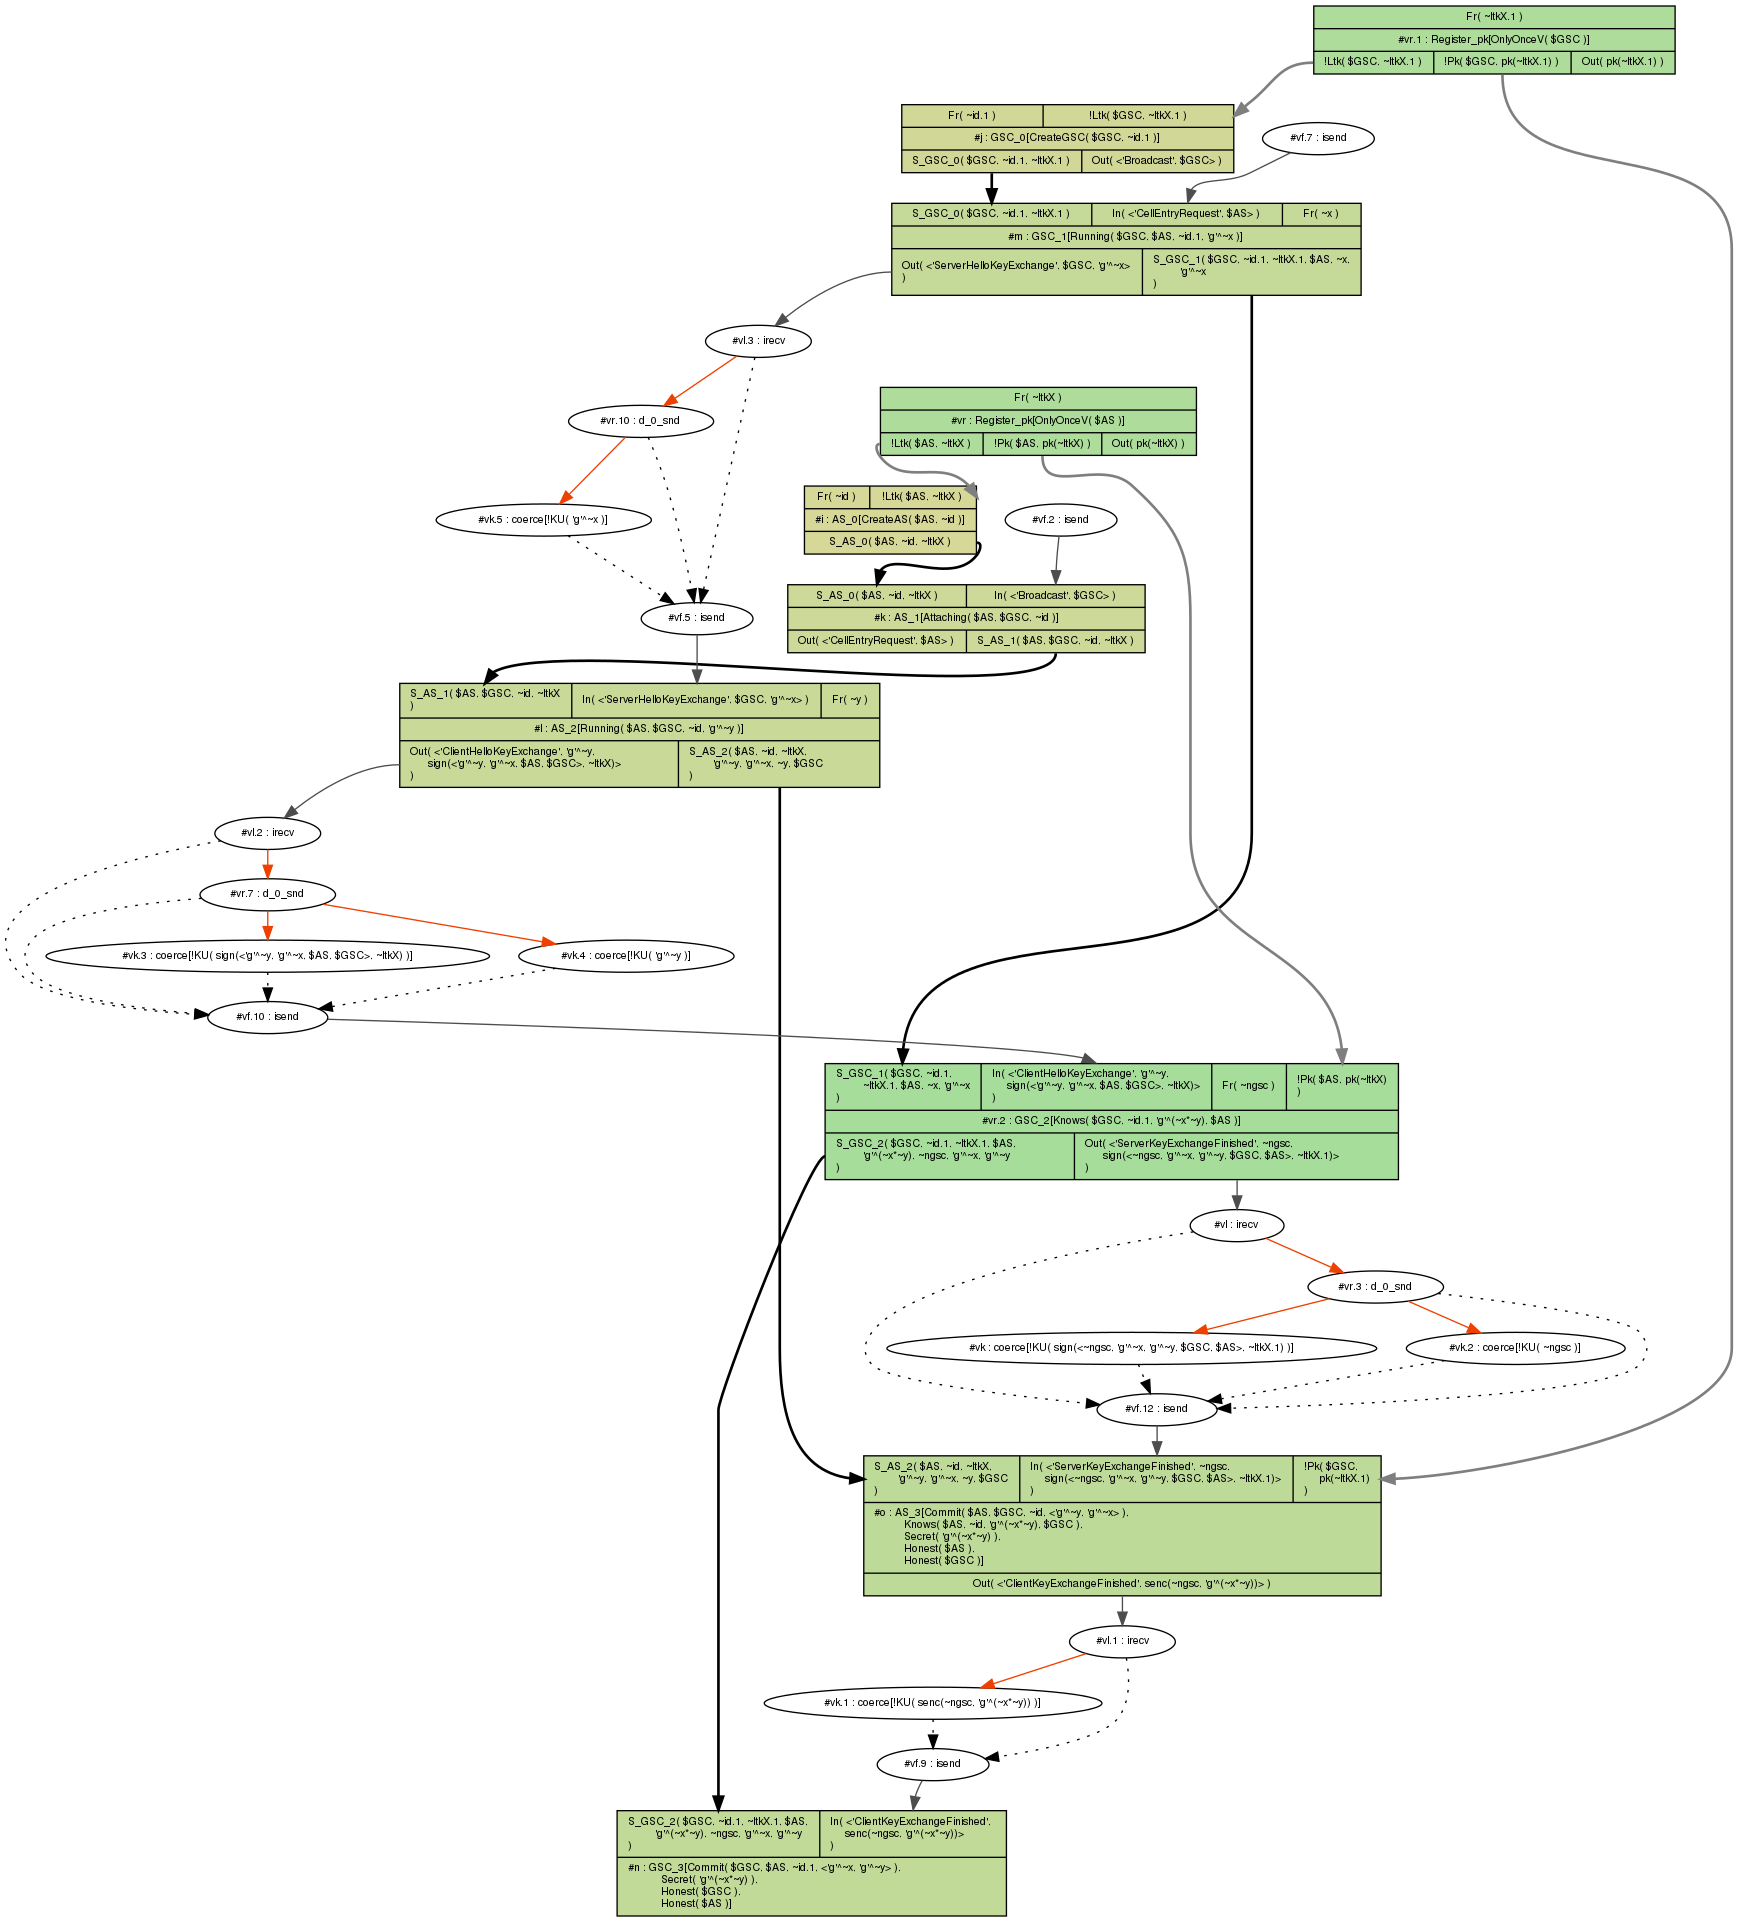
\includegraphics[width=\textwidth]{img/tamarin.png}
		 \caption{Tamarin proof visualization of a successful LDACS MAKE protocol run}
 	\label{fig:figure4}
\end{figure} 

In Figure \ref{fig:figure4} we present the visualization of the proof of the Executable-lemma. It shows a complete trace of the protocol run with both stations AS and GSC engaged. 
It can be seen, that all foreseen messages are being sent and that both stations commit with the same session key.